%% This is my HW 8 solution set.

\documentclass[12pt, leqno]{article}
\usepackage{amsfonts, amsmath, amssymb}
\usepackage{amsbsy}
\usepackage{fancyhdr}
\usepackage{hyperref}
\usepackage{graphicx}
\newcounter{qcounter}
%\usepackage[landscape]{geometry}% http://ctan.org/pkg/geometry
%\usepackage{array}% http://ctan.org/pkg/array
\usepackage[lofdepth,lotdepth]{subfig}
\usepackage[maxfloats=40]{morefloats}
\usepackage{float}
\usepackage{}
\usepackage[english]{babel}
\usepackage{tabularx}
\usepackage{scalerel}
\providecommand{\abs}[1]{\lvert#1\rvert} % absolute value
\providecommand{\normd}{\mathcal{N}} % normal distribution
\providecommand{\norm}[1]{\lVert#1\rVert} % norm
\usepackage{mathtools}
\DeclarePairedDelimiter\ceil{\lceil}{\rceil}
\DeclarePairedDelimiter\floor{\lfloor}{\rfloor}
\newcommand{\macheps}{\epsilon_{\mbox{\scriptsize mach}}}
\usepackage[ampersand]{easylist}
\makeatletter
\newcommand{\distas}[1]{\mathbin{\overset{#1}{\kern\z@\sim}}}%
\newsavebox{\mybox}\newsavebox{\mysim}
\newcommand{\distras}[1]{%
  \savebox{\mybox}{\hbox{\kern3pt$\scriptstyle#1$\kern3pt}}%
  \savebox{\mysim}{\hbox{$\sim$}}%
  \mathbin{\overset{#1}{\kern\z@\resizebox{\wd\mybox}{\ht\mysim}{$\sim$}}}%
}
\makeatother
%\usepackage{pdflscape}


\begin{document}
\pagestyle{fancy}
\lhead{Syed Rahman}
\rhead{CIS6930}

\begin{center}
{\large {\bf Homework 2}} \\
\end{center}

\paragraph{1a}
Note that 
\begin{align*}
\norm{x - \hat{x}_k}_2^2 &= \sum_{k = K}^{\infty} \abs{a_k^*}^2 \\
&\leq  \sum_{k = K}^{\infty} \abs{Ck^{-\beta}}^2 \\
&\leq  \int_{k = K-1}^{\infty} C^2 k^{-2\beta} dk \\
&= \Big[\frac{C^2 k^{-2 \beta + 1}}{-2 \beta + 1}\Big]_{k = K}^{\infty} \\
&= \frac{C^2 K^{- 2 \beta + 1}}{2 \beta - 1}
\end{align*}

\paragraph{1b}
Using the fact that $\beta>1/2$, we solve $K$ for 
\begin{align*}
&\frac{C^2 K^{- 2 \beta + 1}}{2 \beta - 1} \leq \epsilon \\
\iff& K^{- 2 \beta + 1} \leq  \epsilon (2 \beta - 1) / C^2 \\
\iff& \frac{1}{K}^{2 \beta - 1} \leq  \epsilon (2 \beta - 1) / C^2 \\
\iff& {K}^{2 \beta - 1} \geq  C^2 / \epsilon (2 \beta - 1) \\
\iff& {K}^{2 \beta - 1} \geq  C^2 / \epsilon (2 \beta - 1) \\
\iff& {K} \geq  (C^2 / \epsilon (2 \beta - 1))^{1/(2 \beta - 1)} \\
\end{align*}

\paragraph{1c}
For this part we used the image in Figure \ref{flower} reduced to a $5 \times 5$ matrix. As the DCT basis is orthogonal, to find the best $K$-term approximation all we need to do is find the inner products of the DCT basis with the image vector, sort and keep the largest $K$ ceoffcients. Let $a_n^*$ denote the vector of sorted inner products between the DCT basis vectors and the image file. We know that $\abs{a_n^*} \leq Cn^{-\beta} \iff \log(\abs{a_n^*}) \leq \log C  -\beta \log n $. To get an estimate for $\beta$, we fit the following regression model: ${\log{\abs{a_n^*}}} = \alpha - \beta \log n$. This gives us $\beta = 16$ rounded to the nearest integer. Now to find $C$, we smply set it to $\max_{n} = \abs{a_n^*} n^{16}= 57344367963$.

\begin{figure}
\centering
  
\includegraphics[scale=1]{flower.png}
\caption{Picture used for analysis with DCT basis}
\label{flower}
\end{figure}

\begin{verbatim}
size <- 5
flower <- channel((readImage("flower.jpg")),"gray")
flower <- resize(flower,size,size)
kk <- 5
Aflower <- matrix(0,nrow=5,ncol=5)
for(n in 1:kk){
    for(m in 1:kk){
        Aflower[m,n] <- sum(outer(vni(m,1:size,size),
vni(n,1:size,size))*flower)
    }
}
Aflowervec = matrix(Aflower,nrow = 25)
an <- sort(abs(Aflowervec), decreasing = TRUE)
reg1 <- lm(log(an) ~ log(1:25))
C <- max(an*(n^(-16)))
\end{verbatim}

\paragraph{2a}
The code to implement Matching Pursuit:
\begin{verbatim}
MP <- function(x,D,maxiter, eps){
#### to normalize D
    D <- apply(D,2,function(x) {x/sqrt(sum(x^2))})
    nk <- integer(0)
    ak <- integer(0)
#### to initialize xk and Rk
    xk <- rep(0,length(x))
    Rk <- x
    for (iter in 1:maxiter){
        nk <- rbind(nk,which.max(abs(t(D)%*%Rk)))
        ak <- rbind(ak,sum(Rk*D[,nk[iter]]))
        xk1 <- xk + sum(Rk*D[,nk[iter]])*D[,nk[iter]]
        Rk1 <- Rk - sum(Rk*D[,nk[iter]])*D[,nk[iter]]
        if(sqrt(sum((x-xk1)^2))<eps){
            break
        } else {
            xk <- xk1
            Rk <- Rk1
        }        
    }
    return(list(xk=xk1,Rk=Rk1,nk=nk,ak = ak,itr=iter,
err=sqrt(sum((x-xk1)^2))))
}
\end{verbatim}

and the code to implement Orthogonal Matching Pursuit:
\begin{verbatim}
OMP <- function(x, D, maxiter,eps){
#### to normalize D
    D <- apply(D,2,function(x) {x/sqrt(sum(x^2))})
    nk <- integer(0)
    ak <- integer(0)
#### to initialize xk and Rk
    xk <- rep(0,length(x))
    Rk <- x
    uk <- matrix(0,nrow = dim(D)[1], ncol = dim(D)[2])
    nk <- rbind(nk,which.max(abs(t(D)%*%Rk)))
    uk[,1] <- D[,nk[1]]
    ak <- rbind(ak,(sum(Rk*uk[,1])/sum(uk[,1]*uk[,1])))
    xk1 <- xk + (sum(Rk*uk[,1])/sum(uk[,1]*uk[,1]))*uk[,1]
    Rk1 <- Rk - (sum(Rk*uk[,1])/sum(uk[,1]*uk[,1]))*uk[,1]
    if(sqrt(sum((xk1-x)^2))<eps | maxiter ==1){
        return(list(xk=xk1,Rk=Rk1,nk = nk, ak = ak, itr=1,
err=sqrt(sum((x-xk1)^2))))
    }  else    {
            xk <- xk1
            Rk <- Rk1
            #iter = 2
            for (iter in 2:min(dim(D)[2],maxiter)){
                nk <- rbind(nk,which.max(abs(t(D)%*%Rk)))
                sumterm = 0
                for(j in 1:(iter-1)){
                    sumterm = sumterm + (sum(D[,nk[iter]]*uk[,j])/
sum(uk[,j]*uk[,j]))*uk[,j]
                }
                uk[,iter] <- D[,nk[iter]] - sumterm
                ak <- rbind(ak,(sum(Rk*uk[,iter])/sum(uk[,iter]*uk[,iter])))

                xk1 <- xk + (sum(Rk*uk[,iter])/
sum(uk[,iter]*uk[,iter]))*uk[,iter]
                Rk1 <- Rk - (sum(Rk*uk[,iter])/
sum(uk[,iter]*uk[,iter]))*uk[,iter]
                if(sqrt(sum((xk1-x)^2))<eps){
                    break
                } else {
                    xk <- xk1
                    Rk <- Rk1
                }        
            }
            return(list(xk=xk1,Rk=Rk1,nk = nk, ak = ak, itr=iter,
err=sqrt(sum((x-xk1)^2))))          
        }
    }
\end{verbatim}

\paragraph{2b}
To compute the coherence of $D = [I, C]$, we can use the follosing R code:
\begin{verbatim}
mumat <- t(D)%*%D
diag(mumat) <- 0
which(mumat==max(mumat),arr.ind=TRUE)
## so d_3 and d_10 are furthest apart
## coherence in D
mu <- sum(D[,3]*D[,10])
> mu
[1] 0.6324555
\end{verbatim}

As shown we get $\mu = 0.632$.

\paragraph{2 c,d,e,f}
I do all of these parts togerther as it was simplest that way. First to solve basis pursuit we solve the following lasso problem:
\begin{align*}
\min_{a} \frac{1}{2} \norm{x-Da}_2^2 + \lambda \norm{a}_1
\end{align*}
We pick $\lambda$ using 5-fold cross-validation between on an evenly spaced grid between 0.01 and 1.00. This is done using the following R code:
\begin{verbatim}
cv5BP <- function(D,x,nlambda){
foldsize <- floor(length(x)/5)    
err <- matrix(0,nrow = nlambda, ncol = 5)
rndmsmpl <- sample(1:length(x))
folds <- split(rndmsmpl, ceiling(seq_along(rndmsmpl)/foldsize))
for(lambda in 1:nlambda){
    for(i in 1:5){
        a1 <- folds[[i]]
        fit <- lassoshooting(X=D[-folds[[i]],],y=x[-folds[[i]]],
lambda = 0.01*lambda)
        err[lambda,i] <- sum((a1 - D[folds[[i]],]%*%fit$coeff)^2)
    }
}
0.01*which.min(apply(err,1,mean))
}

BP <- function(D,x){
    lambdastar <- cvBP(D,x,100)
    lassoshooting(X=D,y=x,lambda = lambdastar)$coeff
}
\end{verbatim}

The remaining parts of the problem is done using the following code:
\begin{verbatim}
set.seed(12345)
for(N in c(30,60,90,120)){
d <- (N/2)
reps <- 30
normerrMP <- normerrOMP <- normerrBP <- matrix(0,nrow = d, ncol = reps)
for (sprs in 1:d){
    for(MM in 1:reps){
        nz <- sample(x=1:N,size=sprs, replace =FALSE)
        a <- rep(0,N)
        a[nz] <- rnorm(n=sprs)
        C <- vni(0,1:(N/2),(N/2))
        for(i in 1:((N/2)-1)){
            C <- cbind(C,vni(i,1:(N/2),(N/2)))
        }
        I <- diag((N/2))
        D <- cbind(I,C)
        x <- D%*%a
        ahatMP <- rep(0,N)
        ahatOMP <- rep(0,N)
        mp <- MP(x = x, D = D, maxiter = 50, eps = 10^(-5))
        omp <- OMP(x = x, D = D, maxiter = 50, eps = 10^(-5))
        for(i in 1:length(mp$nk)){
            ahatMP[mp$nk[i]] <- ahatMP[mp$nk[i]]+mp$ak[i]
        }
        ahatOMP[omp$nk] <- ginv(D[,omp$nk])%*%omp$xk
        ahatBP <- BP(D,x)
        
        normerrMP[sprs,MM] <- sqrt(sum((ahatMP-a)^2))/sqrt(sum(a^2))
        normerrOMP[sprs,MM] <- sqrt(sum((ahatOMP-a)^2))/sqrt(sum(a^2))
        normerrBP[sprs,MM] <- sqrt(sum((ahatBP-a)^2))/sqrt(sum(a^2))
    }
}
}
\end{verbatim}
We vary $N$ to be $30,60,90, 120$ and set $d = N/2$ in each case. For each of these values we repeat the experiment 30 times and take the average of the relative normed error (RNE) by calculating 
$$
\text{RNE} = \frac{\norm{\hat{a}-a}_2^2}{\norm{a}_2^2} 
$$
and taking the average over the 30 replicates. 

To find $\hat{a}$ for Orthogonal Matching Pursuit we keep track of
which vectors create the maximal angles with the residuals. Suppose
these were 2,3 and 7 at which point the algorithm terminated. Then
$\hat{a}$ is a sparse vector with non-sparse terms in the $2^{nd},
3^{rd} \text{ and } 5^{th}$ positions determined by taking the
generalized inverse of a matrix comprised of the  $2^{nd}, 3^{rd}
\text{ and } 5^{th}$ columns of $D$ and multiplying that by $\hat{x}$,
where $\hat{x}$ denotes the point at which the algorithms
terminate. For Matching Pursuit, we start with a vector of 0's and let
$\hat{a}[n_k] = \hat{a}[n_k]+<R_{n_k},d_{n_k}>$. The plots comparing Matching Pursuit, Orthogonal Matching Pursuit and Basis Pursuit are shown in Figures \ref{fig:ne15m}, \ref{fig:ne30m}, \ref{fig:ne45m}, \ref{fig:ne60m}. Matching Pursuit and Orthogonal Matching Pursuit does very well so long as the sparsity is fairly high (number of non-sparse elements is low) compared to the dimension of the vector being recovered. In fact, for very sparse vectors both of these outperforms Basis Pusruit. However, as the vector becomes denser, it is clear that Basis Pursuit does better than the other methods. 

\begin{figure}
\centering
\subfloat[]
  {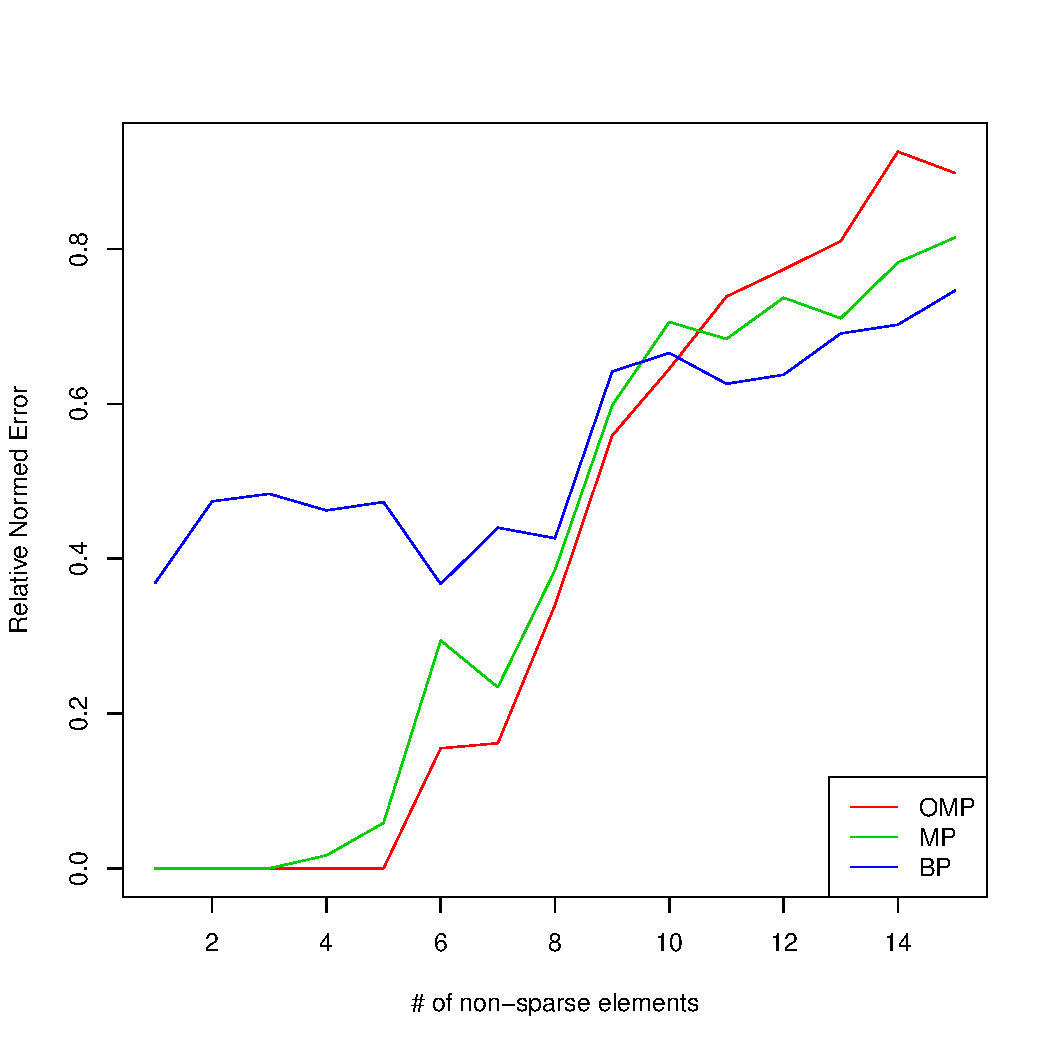
\includegraphics[scale=0.3]{Method2-normerr15.pdf}
\label{fig:ne15m}}
\subfloat[]
  {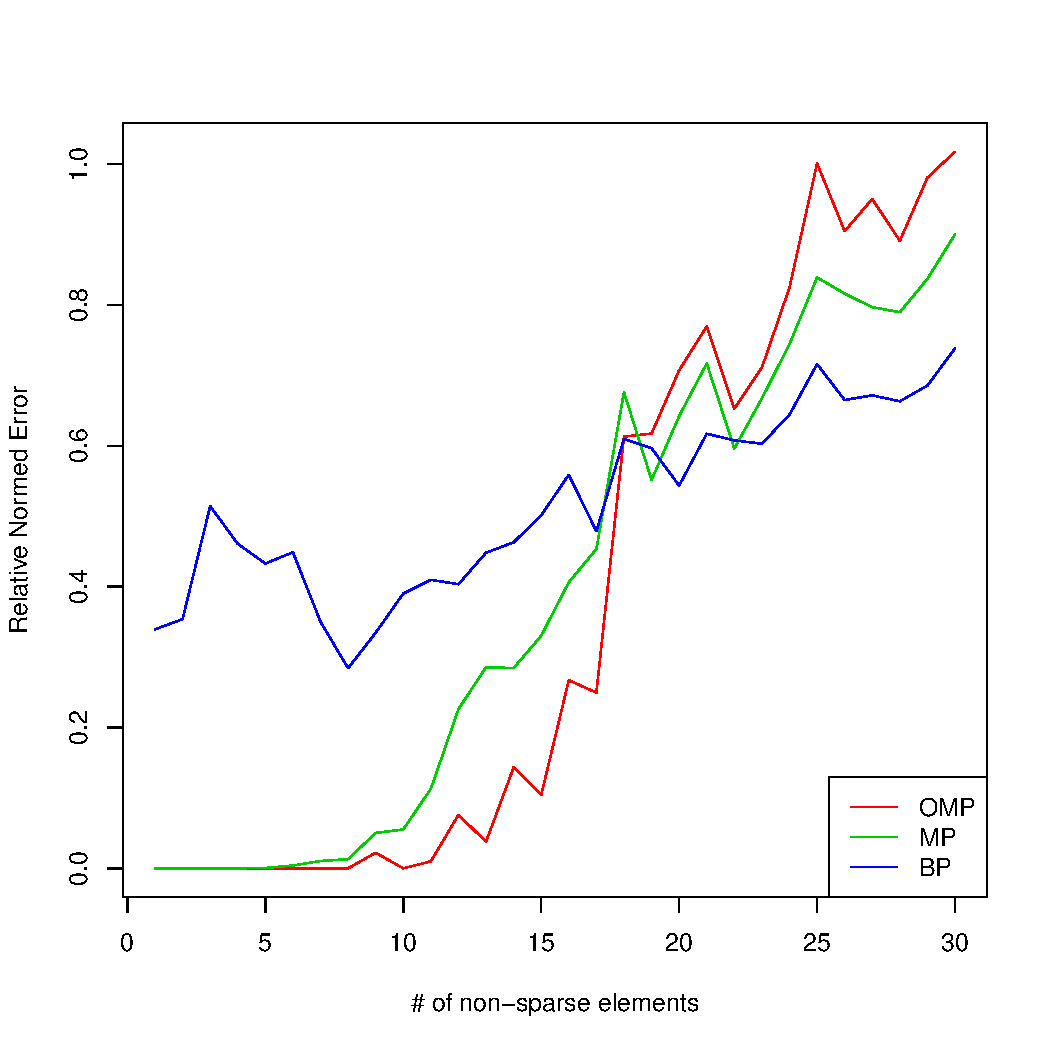
\includegraphics[scale=0.3]{Method2-normerr30.pdf}
\label{fig:ne30m}}
\\
\subfloat[]
  {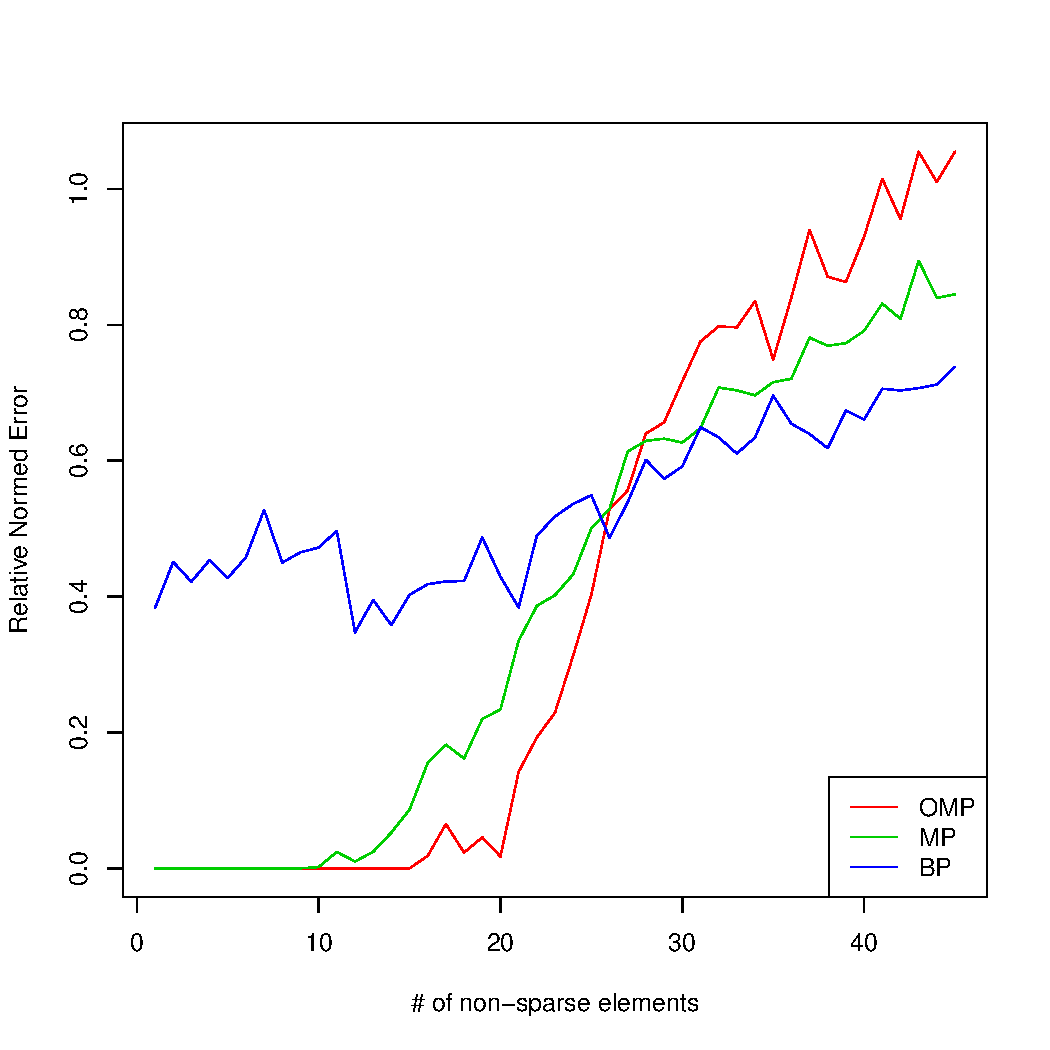
\includegraphics[scale=0.3]{Method2-normerr45.pdf}
\label{fig:ne45m}}
\subfloat[]
  {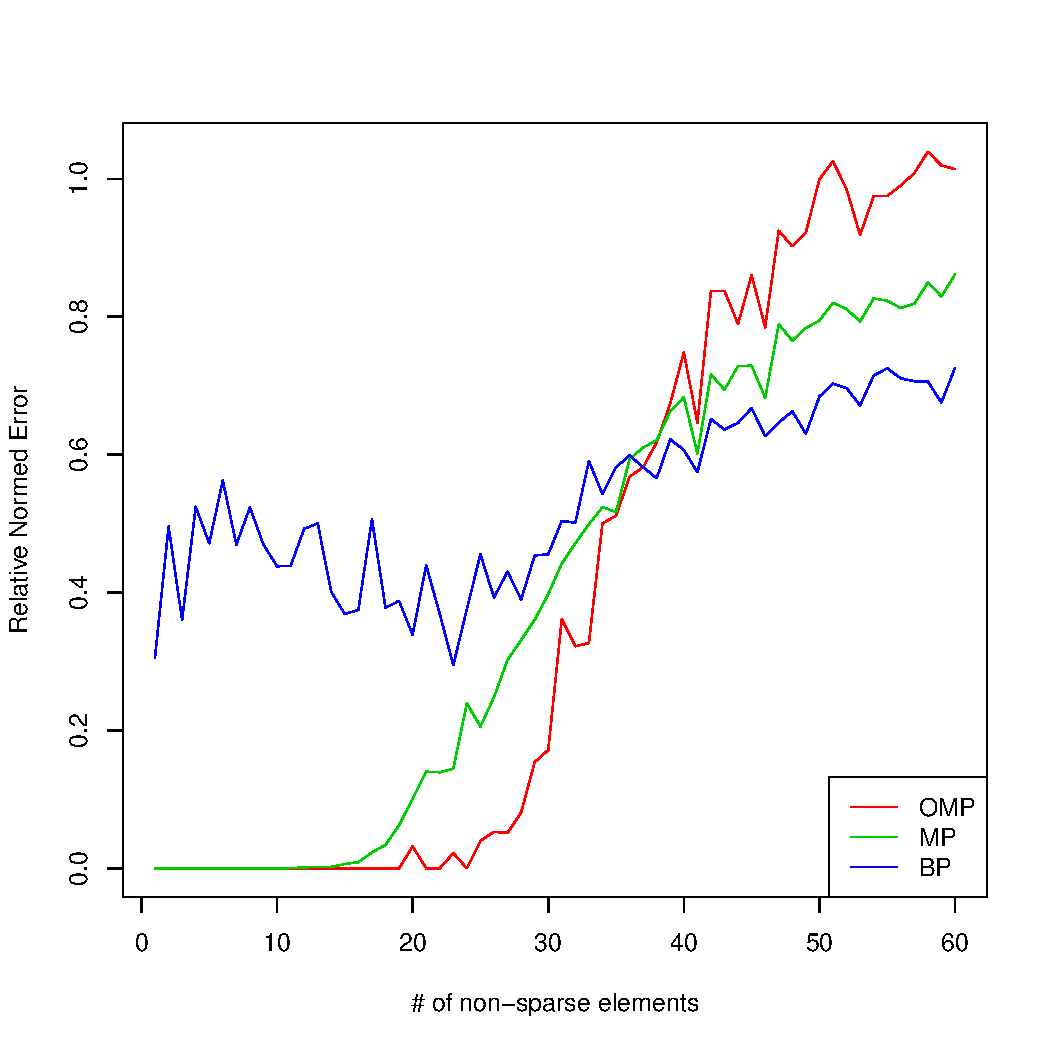
\includegraphics[scale=0.3]{Method2-normerr60.pdf}
\label{fig:ne60m}}
\caption{Relative Normed Errors for Matching Pursuit, Orthogonal Matching Pursuit and Basis Pursuit.  Matching Pursuit and Orthogonal Matching Pursuit performs well when the number of non-sparse elements is low. Basis Pusruit does better than both when the number of non-sparse elements is high.}
\end{figure}

\end{document}